The upgraded Prophet 600 supports three arpeggiator modes.

\scalebox{0.4}{
  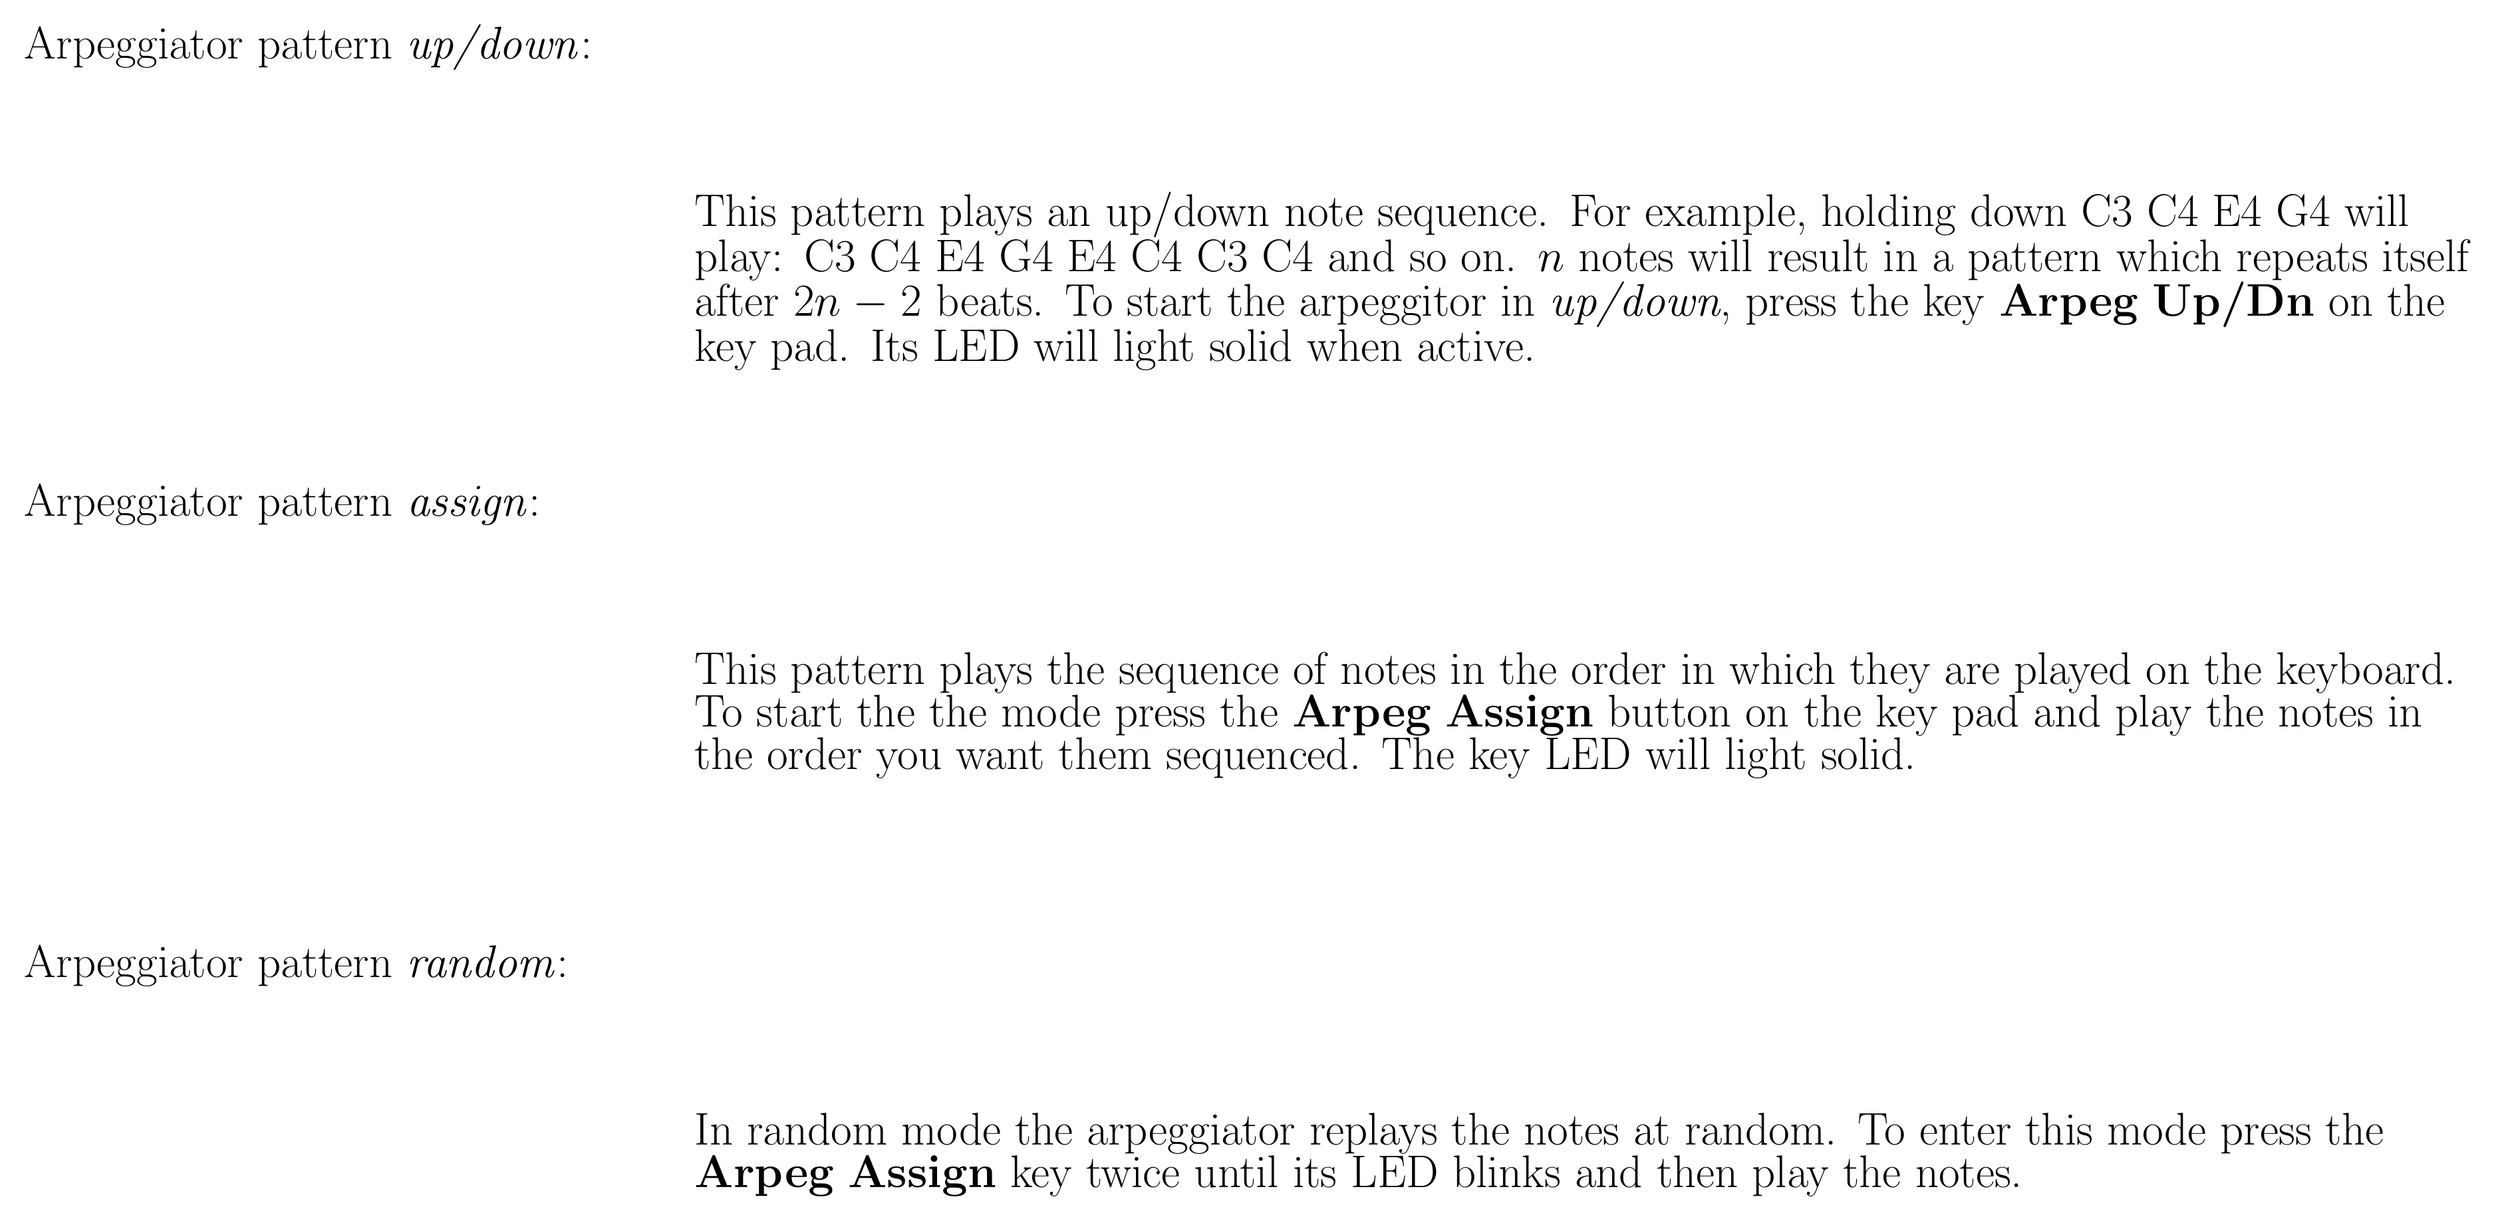
\begin{tikzpicture}[scale=0.8]
  \node[font=\fontsize{26}{22}\selectfont, align=left, outer sep=0.5mm, anchor = north west, text width=30cm] at (0cm,31cm) {Arpeggiator pattern \textit{up/down}:};
  \node[font=\fontsize{26}{22}\selectfont, align=left, outer sep=0.5mm, anchor = north west, text width=34cm] at (16cm,27cm) {This pattern plays an up/down note sequence. For example, holding down C3 C4 E4 G4 will play: C3 C4 E4 G4 E4 C4 C3 C4 and so on. $n$ notes will result in a pattern which repeats itself after $2n-2$ beats. To start the arpeggitor in \textit{up/down}, press the key \textbf{Arpeg Up/Dn} on the key pad. Its LED will light solid when active.};
    \arpsqbuttons{1cm, 22cm}{U}{}
    
  \node[font=\fontsize{26}{22}\selectfont, align=left, outer sep=0.5mm, anchor = north west, text width=30cm] at (0cm,20cm) {Arpeggiator pattern \textit{assign}:};
  \node[font=\fontsize{26}{22}\selectfont, align=left, outer sep=0.5mm, anchor = north west, text width=34cm] at (16cm,16cm) {This pattern plays the sequence of notes in the order in which they are played on the keyboard. To start the the mode press the \textbf{Arpeg Assign} button on the key pad and play the notes in the order you want them sequenced. The key LED will light solid.};
    \arpsqbuttons{1cm, 11cm}{A}{}

    
  \node[font=\fontsize{26}{22}\selectfont, align=left, outer sep=0.5mm, anchor = north west, text width=30cm] at (0cm,9cm) {Arpeggiator pattern \textit{random}:};
  \node[font=\fontsize{26}{22}\selectfont, align=left, outer sep=0.5mm, anchor = north west, text width=34cm] at (16cm,5cm) {In random  mode the arpeggiator replays the notes at random. To enter this mode press the \textbf{Arpeg Assign} key twice until its LED blinks and then play the notes.};
    \arpsqbuttons{1cm, 0cm}{A}{A}
  \end{tikzpicture}
}

Note that compared the version 2.0 and 2.1 RC3 the up/down pattern and the random pattern have been changed. In these versions the lowest and highest note in the up/down pattern were played twice, in version \version they are only played once. Formerly, a single note could be repeated two or more times in the random pattern. Now a note is never repeated (unless there is only one note to play).

It is possible to sync the LFO to the arpeggiator using the additional patch parameter \clocksync, see section \ref{sync}.

\textbf{Latch mode}

With all arpeggiator modes, press the \record button on the key pad to enter the arpeggiator latch mode where played notes are held, e.g. continue to be played after they are released. The LED of the \record button will light solid. Playing additional notes in this mode will add them as additional notes to the existing sequence, up to a maximum of 128 notes. To clear the notes from the sequence, press the \record button to switch the latch mode off. The LED of the Record button will go off.

The foot switch has the same function as pressing \record while the arpeggiator is running, e.g. it toggles the arpeggiator latch mode as indicated by the \record LED. 

\textbf{Transpostion}

The arpeggiator pattern can be transposed on the fly. To do so use the keyboard in shifted or shift-locked mode, see section \ref{transposition}.

\textbf{Controlling the arpeggiator using MIDI}

It is possible to input notes into the arpeggiator via MIDI. The MIDI behaviour in this context depends on the MIDI mode (\textit{local on} or \textit{local off}, see section \ref{midiintegration} in the following way when the arpeggiator is running:

\begin{itemize}
  \item \textit{local on}: Keys played on the keyboard are entered into the arpeggiator. Transposition works normally. MIDI notes sent to the Prophet 600 play normally, e.g. they are not sent to the arpeggiator but play  on top of the running arpeggiator.
  \item \textit{local off}: Keys played on the keyboard are not entered into the arpeggiator but are sent out as MIDI in the normal way. Transposition works normally from the keyboard. MIDI notes sent to the Prophet 600 are input into the arpeggiator. MIDI cannot play normally on top of the arpeggiator. 
\end{itemize}

\textbf{Trouble shooting}

If the arpeggiator is activated and keys are held down or have been latched and still no sound plays, then it is worth checking the following potential reasons: Is the sync set to \textit{internal} and is the \clock greater than zero? If the sync is not \textit{internal} does the instrument receive a clock, e.g. via MIDI on the correct channel or via tape in? If the instrument in \textit{local on} mode (see section \ref{midiintegration})?
